%%%%%%%%%%%%%%%%%%%%%%%%%%%%%%%%%%%%%%%%%
% University Assignment Title Page 
% LaTeX Template
% Version 1.0 (27/12/12)
%
% This template has been downloaded from:
% http://www.LaTeXTemplates.com
%
% Original author:
% WikiBooks (http://en.wikibooks.org/wiki/LaTeX/Title_Creation)
%
% License:
% CC BY-NC-SA 3.0 (http://creativecommons.org/licenses/by-nc-sa/3.0/)
% 
% Instructions for using this template:
% This title page is capable of being compiled as is. This is not useful for 
% including it in another document. To do this, you have two options: 
%
% 1) Copy/paste everything between \begin{document} and \end{document} 
% starting at \begin{titlepage} and paste this into another LaTeX file where you 
% want your title page.
% OR
% 2) Remove everything outside the \begin{titlepage} and \end{titlepage} and 
% move this file to the same directory as the LaTeX file you wish to add it to. 
% Then add \input{./title_page_1.tex} to your LaTeX file where you want your
% title page.
%
%%%%%%%%%%%%%%%%%%%%%%%%%%%%%%%%%%%%%%%%%
%\title{Title page with logo}
%----------------------------------------------------------------------------------------
%	PACKAGES AND OTHER DOCUMENT CONFIGURATIONS
%----------------------------------------------------------------------------------------

\documentclass[12pt]{article}
\usepackage[english]{babel}
\usepackage[utf8x]{inputenc}
\usepackage{amsmath}
\usepackage{graphicx}
\usepackage[colorinlistoftodos]{todonotes}
\usepackage{listings}
\usepackage{xcolor}
\usepackage{diagbox}
\usepackage{array}
\usepackage{color}


\definecolor{dkgreen}{rgb}{0,0.6,0}
\definecolor{gray}{rgb}{0.5,0.5,0.5}
\definecolor{mauve}{rgb}{0.58,0,0.82}

\lstset{frame=tb,
	language=Java,
	basicstyle=\small,
	aboveskip=3mm,
	belowskip=3mm,
	showstringspaces=false,
	columns=fullflexible,
	numbers=none,
	numberstyle=\tiny\color{gray},
	keywordstyle=\color{blue},
	commentstyle=\color{dkgreen},
	stringstyle=\color{mauve},
	breaklines=true,
	postbreak=\raisebox{0ex}[0ex][0ex]{\color{red}$\hookrightarrow$\space},
	breakatwhitespace=true,
	tabsize=3
}

\begin{document}

\begin{titlepage}

\newcommand{\HRule}{\rule{\linewidth}{0.5mm}} % Defines a new command for the horizontal lines, change thickness here

\center % Center everything on the page
 
%----------------------------------------------------------------------------------------
%	HEADING SECTIONS
%----------------------------------------------------------------------------------------

\textsc{\LARGE Politenico di Milano}\\[1.5cm] % Name of your university/college
\textsc{\Large Dipartimento Elettronica, Informazione e Bioingegneria}\\[0.5cm] % Major heading such as course name
\textsc{\large HEAPLab Project Report}\\[0.5cm] % Minor heading such as course title

%----------------------------------------------------------------------------------------
%	TITLE SECTION
%----------------------------------------------------------------------------------------

\HRule \\[0.4cm]
{ \huge \bfseries EdgeCloudSim Report}\\[0.4cm] % Title of your document
\HRule \\[1.5cm]
 
%----------------------------------------------------------------------------------------
%	AUTHOR SECTION
%----------------------------------------------------------------------------------------

\begin{minipage}{0.4\textwidth}
\begin{flushleft} \large
\emph{Author:}\\
Zhang \textsc{Qiaolun} % Your name
\end{flushleft}
\end{minipage}
~
\begin{minipage}{0.4\textwidth}
\begin{flushright} \large
\emph{Supervisor:} \\
Michele \textsc{Zanella} % Supervisor's Name
\end{flushright}
\end{minipage}\\[2cm]

% If you don't want a supervisor, uncomment the two lines below and remove the section above
%\Large \emph{Author:}\\
%John \textsc{Smith}\\[3cm] % Your name

%----------------------------------------------------------------------------------------
%	DATE SECTION
%----------------------------------------------------------------------------------------

{\large \today}\\[2cm] % Date, change the \today to a set date if you want to be precise

%----------------------------------------------------------------------------------------
%	LOGO SECTION
%----------------------------------------------------------------------------------------

\includegraphics[width=100pt]{heaplogo.pdf}\\[1cm] % Include a department/university logo - this will require the graphicx package
 
%----------------------------------------------------------------------------------------

\vfill % Fill the rest of the page with whitespace

\end{titlepage}




\begin{abstract}
The simulation tool EdgeCloudSim provides environment to simulate edge computing scenarios, which can be used to conduct experiments that considers both computational and networking resources. However, the application allocated and scheduled in the system is atomic, which means the application cannot be divided and can only be allocated in one devices. But seperating the application into multiple kernels and distributing them to edge servers in the vicinity really counts because edge server is usually resource limited and may not capable to execute the application. In this project, the atomic application simulation in EdgeCloudSim is extended into thread-based application, which provides a more realistic simulation of computation and networking in edge computing.
\end{abstract}

\section{Introduction}

Edge Computing is a new computing paradigm which utilize the resources near the data source and collabrates with cloud computing to provide better services to the user. EdgeCloudSim is a simulation tool which can simulate edge computing and cloud computing scenarios which combine Edge Computing and Cloud Computing. EdgeCloudSim. EdgeCloudSim is extended from CloudSim and uses the discrete event management framework to simulate the dispatching and scheduling of applications. 


The core simulation process is a loop function which checks the events related to all the entities and processes the event. Each entities can process different kinds of events. Figure 1 shows the relations between the EdgeCloudSim modules. The SimSettings class in core simulation modules will load and store all the simulation settings information, which includes the application parameters, the edge server settings, the simulation environment settings. The load generator module will utilize the information in SimSettings instance to generate applications that will be scheduled. Mobility module generates the position of each application when generating applications. Then the simulation of edge computing scenarios starts and the program will goes into a loop. At each cycle, the simulation will check whether there are some events starts at that time. MobileDeviceManager will check if there are new applications that need to be submitted at that time. The sttart time of each application is defined in load generator module before. If there is new applications that need to be submitted, edge orchestrator module will utilize the specified allocation strategy to calculate the virtual machine in a server to execute the application. Then MobileDeviceManager class will utilize the calculated information in edge orchestrator module to submit the application to CloudSim (Base). The entity related to scheduling applications in the virtual machines is defined in CloudSim.


\begin{figure}
	\centering
	\includegraphics[width=1\textwidth]{./figures/1-edgecloudsim_diagram.png}
	\caption{\label{fig:module}Module relationship between modules in EdgeCloudSim.}
\end{figure}


\section{Problem Statement}
In EdgeCloudSim, the application is atomic and can only be executed in one edge devices. However, some applications can be divided into multiple kernels and simulate the execution of these kernels really counts. Since single edge sever is resources-limited and may not have enough resoruces to execute the application. But executing the application in the cloud may lead to time-delay and even miss the deadline of the application.  Consequently, application is divided into multiple small kernels, which are distributed into multiple edge server. So it is necessary to provide kernel-based application feature to simulate edge computing scenarios. The modules that need to be modified or added are listed as follows:

\begin{enumerate}
	\item core: change the core classes related to load settings, managing events in the system and store status of kernel-based applications. This module also defines a KernelBasedAppliationStatus.java class to store the status of all the applications.
	\item edge\_clinet: define the classes for kernel.
	\item mobility: change the mobility module to adapte to generate the positions for kernel-based applications.
	\item task\_generator: generate kerne\_based applications
	\item utils: define the classes related to kernel-based applications. Moreover, SimLogger.java are modified to calculate the simulation results for kernel-based applications.
	\item config: the config file applications.xml are redifned for kernel-based applications.
\end{enumerate}


\section{Design and Implementation}

\subsection{Kernel-Based Application Design}
In EdgeCloudSim, application is atomic and cannot be divided into smaller kernels. In this project, kenel-based application is introduced into this simulation tool. Kernel-based application is composed of a single kernel or multiple kernels. And the kernel is distinguised by kernel ID in this implementation. The original application.xml file are modified to represent the parameters for kernel-based application. The Applications.xml describes the types and parameters of applications in the simulation. Parameters in the original Applications.xml file of EdgeCloudSim is not explained, which makes it difficult to understand the meaning of these parameters.  The meanings of the some important parameters are listed as follows:

\begin{enumerate}
	\item usage\_percentage: The usage percentage here is used to decide the percentage of this type of application in all of the applications generated. So add up usage\_percentage field in the applications.xml, we can get 100 because we have sumed up all the percentages of all applications.
	\item prob\_cloud\_selection: The probability that we choose the cloud to execute the applications.
	\item active\_period: In active period, the edge devices can generate new applications.
	\item idle\_period: In idle period, the edge devices can not generate new applications.
\end{enumerate}

A sample of new application.xml shows as follows:
\lstinputlisting{./code/Applications.xml}


The implementation of kernel-based application in EdgeCloudSim is developed by the abstraction of kernels. The original atomic task in EdgeCloudSim are changed to a kernel. An application can have one or multiple kernel. The kernel id is unique in this simulation tool. When an kernel-based application that have multiple kernels is created, an KernelBasedApplication.java class is instanciated and stores the kernel id of all the kernels that belongs to it. Moreover, this class handles the dependencies between the kernels in this application in runtime. All the instance of KernelBasedApplication is stored in a singleton instance of KernelBasedApplicationStatus.java. When we want to query or change the states of kernel-based application, we use the function in the singleton instance of KernelBasedApplicationStatus.java.

Adding the events of submitting kernels in runtime is required because we choose only submit a kernel to virtual machine when its dependencies has been met. This requirement is implemented using the event-driven simulation mechanism in CloudSim. In the CloudSim, so  When a Cloudlet(kernel) is finished, it will send a CLOUDLET\_RETURN event to DatacenterBroker. In EdgeCloudSim, this event will be sent to MobileDeviceManager. Then processCloudletReturn function will be triggered. So when a kernel is finished, the kernels belongs to the same kernel-based applications will be checked. If there are kernels whose dependencies has been met now, it will be submitted to the VM at this time. The submit of kernel are based on the schedule function. We implement these functions in MobileDeviceManager class. What the scheduling function does is actually creating events for the entities. The entities in EdgeCloudsim are listed as follows:
\begin{enumerate}
	\item SimManager: public class SimManager extends SimEntity
	\item MobileDeviceManager: public abstract class MobileDeviceManager  extends DatacenterBroker
	\item EdgeOrchestrator: public abstract class EdgeOrchestrator extends SimEntity
\end{enumerate}


\begin{figure}
	\centering
	\includegraphics[width=1\textwidth]{./figures/2-updateCloudletProcessing.pdf}
	\caption{\label{fig:cloudletProcessing}Call hierarchy of function updateCloudletProcessing.}
\end{figure}

Although we can access the kernel ID of kernels that needs to be submitted, the MobileDeviceManager cannot have access to the load generator. So send an event of submitting these kernels to SimManager. The following code shows the process that sends the event to SimManager in MobileDeviceManager.
\lstinputlisting{./code/processCloudletReturn.txt}

The  following code shows how the kernels is submitted in SimManager. Since the kernel needs to be allocated to specific virtual machines in a chosen host in runtime, the kernel is instanciated at this time. First we will retrieve KernelProperty instance related to this kernel, then pass it into the function submitKernel in class MobileDeviceManager. Actually now goes back to MobileDeviceManager instance.
\lstinputlisting{./code/createKernelInSimManager.txt}

The following code shows a small part of the submitKernel function in MobileDeviceManager.
\lstinputlisting{./code/submitKernel.txt}


\subsection{Allocation of Kernel-Based Application}
The allocation of kernel-based application is based on the following steps.
First, the parameters of different kinds of applications is loaded into SimSettings.java and stored in the following variables:
\begin{enumerate}
	\item private double[][] applicationLookUpTable: store the parameters of applications.
	\item private double[][] kernelInKernelBasedAPPLookUpTable: store the parameters of kernels in kernel-based application
\end{enumerate}

Then load generator will generate all the applications and set their start time. The following code only contains some important lines from LoadGenerator. Singleton KernelBasedApplicationStatus stores all the runtime information of the kernel-based applications. All LernelBasedApplication instance are  stored in KernelBasedApplicationStatus. At this time, we only create the kernel ID and create an kernelProperty instance for each kernel to store its information. An instance of Kernel.java will be created later and the runtime information will be stored in the kernel instance.  Moreover, a kernelPropertyList is created and stores the proeprty of al the kernels.
\lstinputlisting{./code/loadGenerator.java}

When simulation starts, SimManager will loop over  kernelPropertyList. It will check whether the kernel belongs to a kernel-based application that have multiple kernels. If it is, the kernels that dependencies have been met will be extracted. Then event of submitting these kernels at the start time of the applicaions that they belong to will be added for these kernels. If it is an application with a single kernel, an event of submitting this kenel at the start time of the corresponding applications will be added. The code are shown as follows.
\lstinputlisting{./code/SimManagerSubmit.java}

When some kenels in kernel-based applications ends, there may be some kernels that can be submitted. The dependencies between kernels are maintained in KernelBasedApplicationStatus. When MobileDeviceManager knows some kernels ends. It will check whether the task is a kernel in kernel-based applications that have multiple kernels. If it is, Then it will check whether there are other kernels can be submitted after the ending of this kernel. If there are such kernels, the kernels will sbumitted. How to submit these kernels are described at the end of section 3.1.

\subsection{Mapping between Kernel-Based Application and it's kernel}


\subsection{Classes Implementation}

\subsubsection{KernelProperty.java}
KernelProperty.java are changed from the taskProperty.java in EdgeCloudSim. The kernelProperty.java are instantiated in load generator module. And the kernel ID are also generated in load generator and stored in KernelProperty.java.The fields in KernelProperty.java are listed as follows:
\lstinputlisting{./code/KernelProperty.java}


\subsubsection{Kernel.java}
Kernel.java are changed from Task.java in EdgeCloudSim. Kernel.java extends Cloudlet.java class from CloudSim. In CloudSim, Cloudlet is the task scheduled and executed. Kernel will be submitted to CloudSim base. KernelProperty.java are instantiated using KernelProperty.java. Some fields in Kernel.java are determined in run-time. For example, mobileDeviceId, hostIndex, vmIndex, datacenterId are determined in runtime using the scheduling and dispatching algorithm.
\lstinputlisting{./code/Kernel.txt}



\subsubsection{KernelBasedApplicationSettings.java}
KernelBasedApplicationSettings.java is used to store the task dependency. The following code shows the fields in KernelBasedApplicationSettings.java. Table 1 shows  an example of dependency in KernelBasedApplicationSettings.java. If kernel 1 depends on kernel 2, then the value whose row is 1 and column is 2 is 1. Otherwise, the value in the table is 0. In the example given by the table, kernel 1 and kernel 2 can start at the start time of the application. Kernel 3 can only start after the end of kernel 1. Kernel 4 can only start after the end of kernel 1 and kernel 2.

\lstinputlisting{./code/KernelBasedApplicationSettings.java}


\begin{table}
	\centering
	\begin{tabular}{c|c|c|c}
	\hline 
	0 & 0  & 0 & 0\\
	\hline  
	0 & 0 & 0 & 0\\
	\hline
	1 & 0  & 0 & 0\\
	\hline  
	1 & 1 & 0 & 0\\
	\hline 
	\end{tabular}
	\caption{\label{tab:widgets}An example of dependency in KernelBasedApplicationSettings.java.}
\end{table}


\subsubsection{KernelBasedApplication.java}
This class is created in load generator. When we initialize the simulation, all the application that will be created in the simulation is determined and this class is instanciated. This class is used to store the runtime status of the kernel-based application. Some important fields of this class are shown as follows:
\lstinputlisting{./code/KernelBasedApplication.java}

\subsubsection{KernelBasedApplicationStatus.java}
This class is a singleton and stores all the instance of KernelBasedApplication.java. Each module can access this class using the static function getInstance in KernelBasedApplicationStatus.java class. Some important fields of this class are shown as follows:
\lstinputlisting{./code/KernelBasedApplicationStatus.java}

\subsubsection{SimLogger.java and LogItem.java}


A new field kernelId is added to the LogItem.java class to map map the kernel to the log LogItem.
\lstinputlisting{./code/LogItem.java}

\subsection{Simulation Workflow}

The simulation works in the following steps. First SimManager will use the class SimSettings to load the settings about the application types, edge server, and some other parameters. 

The generation of applications are in two phase. In the first phase, SimManager will utilize LoadGenerator to generate the applications that will be scheduled in the simulation. In this process, LoadGenerator will use Possion process to get the arrival time of each applications and use the parameters in SimSettings to generate the positions of each applicaion. Then comes to the second phase, it's a loop to submit the kernels in the application to be scheduled. The loop ends when the simulation comes to the end of the simulation time. In each loop, SimManager will check its the events that needs to be processed at that time. Before the start of the loop, there are two types of events that are determined. The first type is the kernel in applications that only have one kernel. Their start time are determined so the submitting those kernel at the start time of the kernel-based application is added to the events of SimManager. The other type of events is related to the kernels of kernel-based application. The  events of submitting kernels that do not have any dependencies in kernel-based applications  will be added. When some kernels finishes, some other kernels that depends on it can be submitted at that time. The events of submitting these kernels will be  added at run time.

\begin{figure}
	\centering
	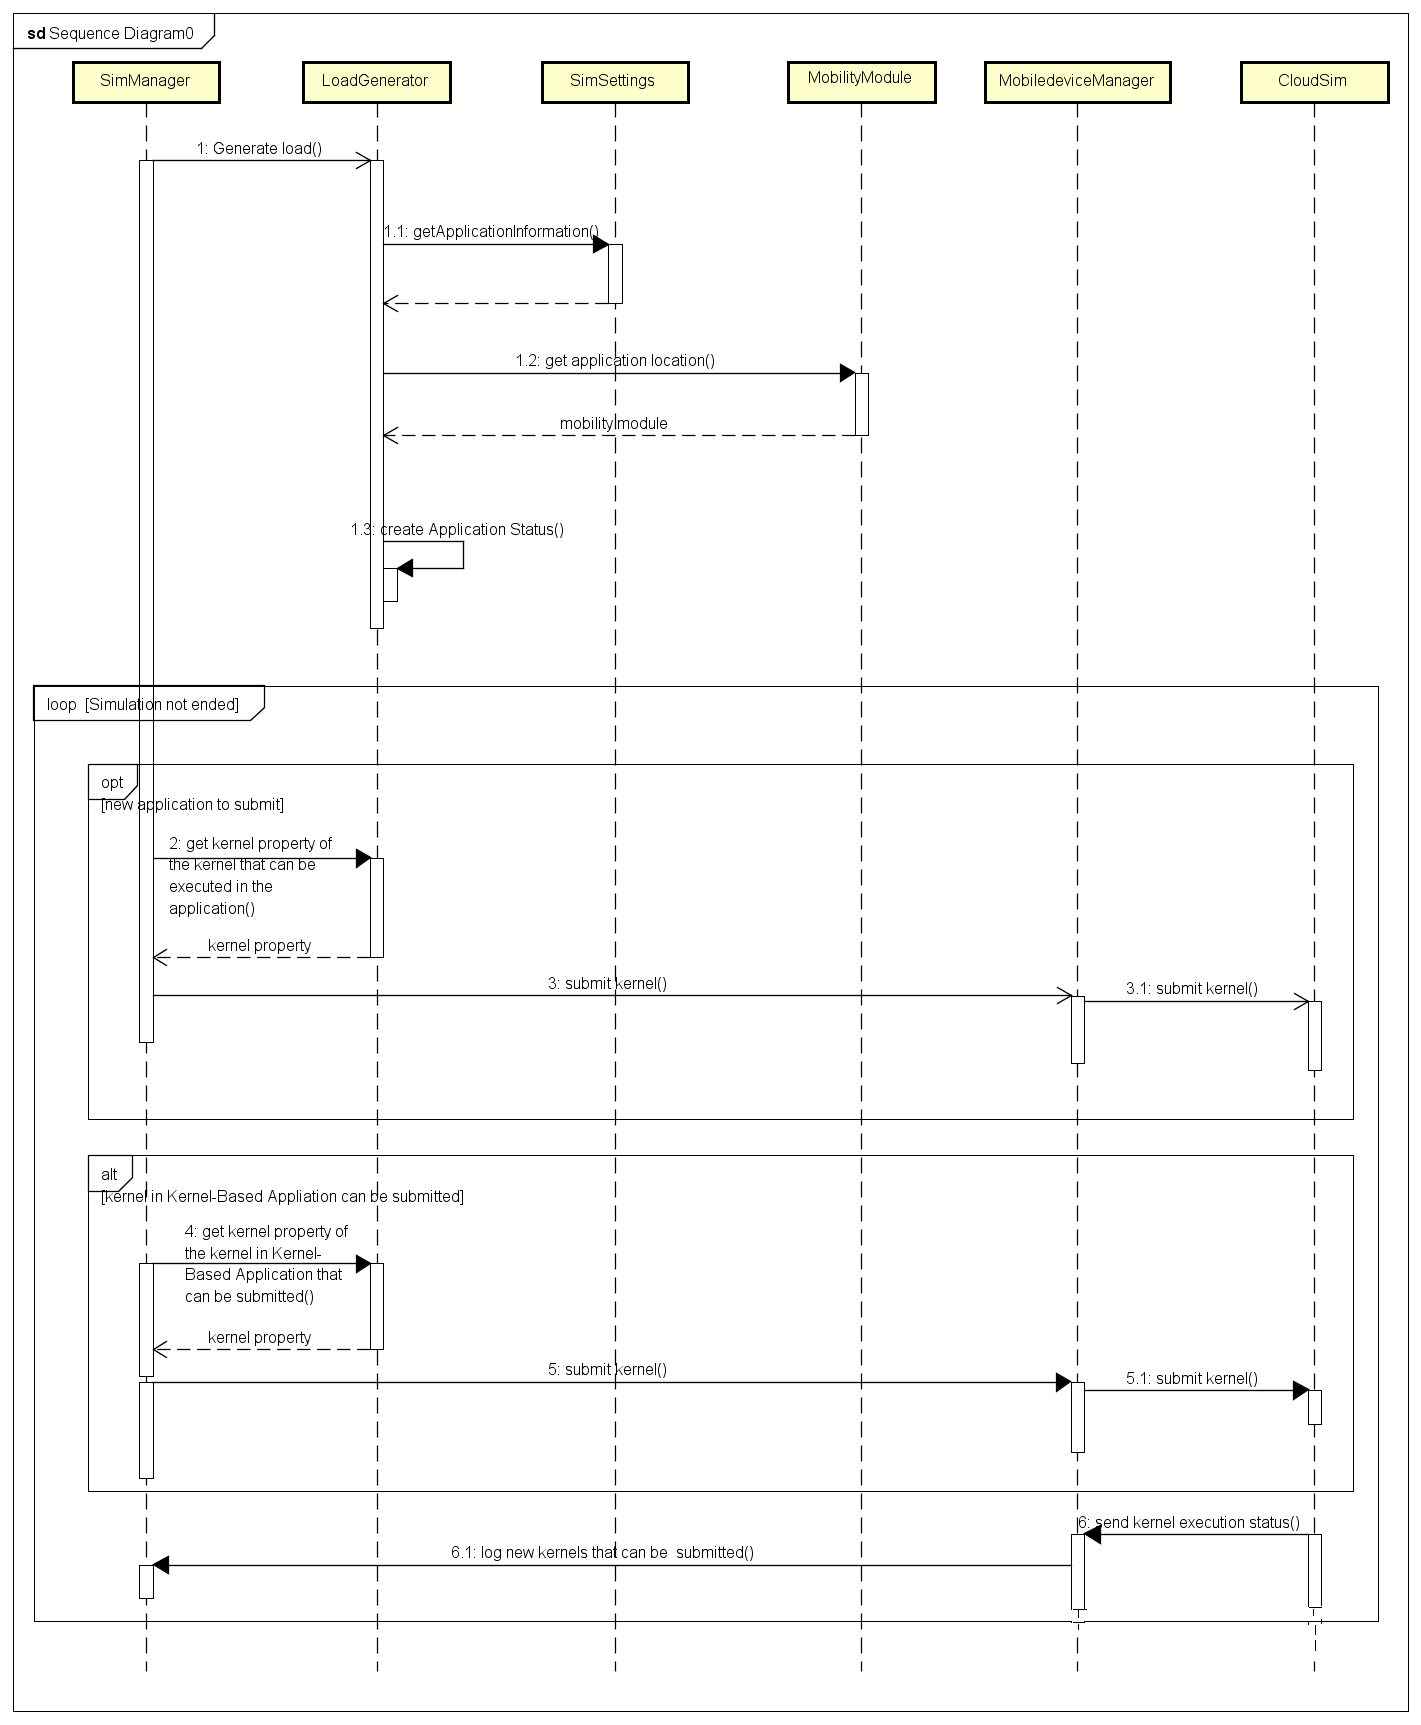
\includegraphics[width=1\textwidth]{./UML/sequence-diagram-create-kernel.png}
	\caption{\label{fig:create-kernel}Modules and functions related to create and submit kernel.}
\end{figure}

After the kernel is submitted, it is scheduled in CloudSim. Figure  shows the Cloudlet processing update process in CloudSim. The original in the paper about CloudSim is wrong. Figure 2 is the fixed figure about Cloudlet processing update process. EdgeCloudSim will decide the device(DataCenter in CloudSim), host, and virtual machine to submit the kernel in runtime. After submitting the kernel, the schedulling process in the virtual machines is handled by CloudSim.

\begin{figure}
	\centering
	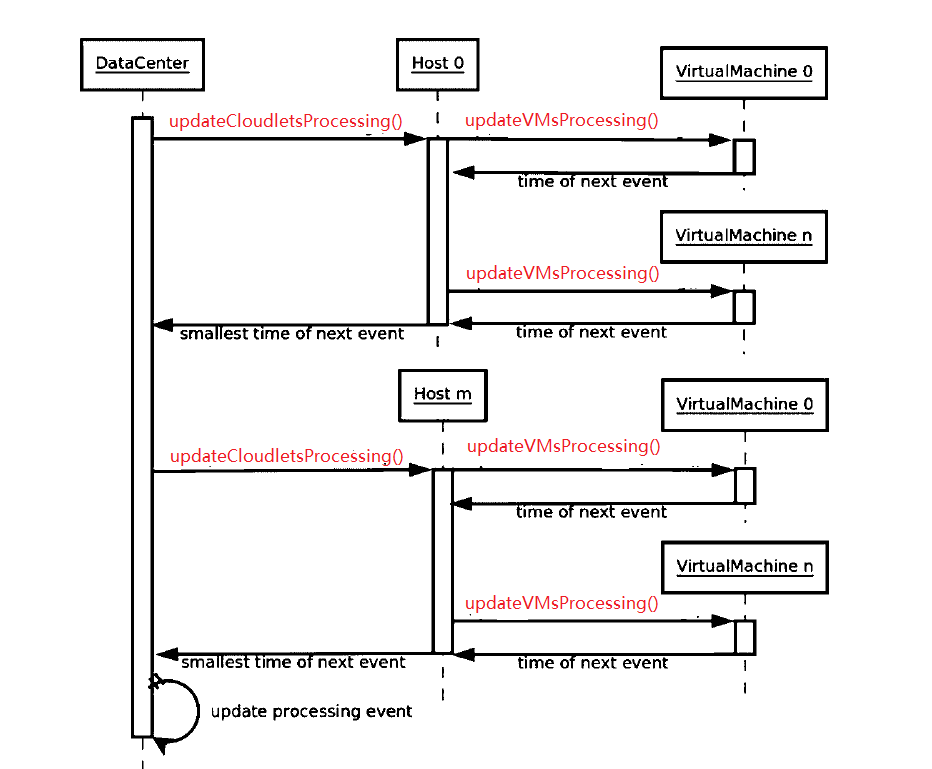
\includegraphics[width=1\textwidth]{./figures/3-processingSequence.png}
	\caption{\label{fig:processingSequence}Cloudlet processing update process.}
\end{figure}

\section{Experimental Results}
In this section, we did some experiment. We test the failure rate.

\section{Conclusions}


\section{Future Works}



\end{document}